\section{Results}

\subsection{Data and subsampling}

More than 2.6 million optical coherence tomography (OCT) images were extracted
from the imaging database and linked to clinical data from the electronica
medical records (EMR). A total of 48,312 normal OCT scans and 52,690 AMD scans
met the inclusion criteria for use in the training set. At the outset, a test
set was set aside comprising of 9,493 images, to be used only for evaluation of
the training procedure once it is done.

To test the effect of sample size on accuracy of classification with a DL
network, random subsets of 4\%, 8\%, 16\%, 32\%, 64\%, and 100\% were created
from the full dataset, and training was conducted using these different subset
sizes. The breakdown in the number of images in each subset is described in
Table \ref{table_counts}.

\begin{table}[!t]
%% increase table row spacing, adjust to taste
\renewcommand{\arraystretch}{1.1}
% if using array.sty, it might be a good idea to tweak the value of
% \extrarowheight as needed to properly center the text within the cells
\caption{Average image counts for each subset condition}
\label{table_counts}
\centering
%% Some packages, such as MDW tools, offer better commands for making tables
%% than the plain LaTeX2e tabular which is used here.
\begin{tabular}{ccccc}
\hline
\multirow{2}{*}{Subset Percentage} & \multicolumn{2}{c}{Training} & \multicolumn{2}{c}{Validation}  \\
	 & Normal & AMD & Normal & AMD \\
\hline
4\%   & 1,355 & 1,338 & 398 & 374 \\
8\%   & 2,637 & 2,503 & 837 & 815 \\
16\%   & 5,983 & 5,457 & 1,575 & 1,659 \\
32\%   & 10,376 & 10,256 & 3,609 & 3,565 \\
64\%   & 22,692 & 20,574 & 7,247 & 7,059 \\
100\%   & 36,515 & 32,204 & 12,028 & 10,762 \\
\hline
\end{tabular}
\end{table}

\subsection{Learning with different size subsamples}

To assess the robustness of the results to the random selection of specific
images, random subsamples of each one of these proportions were drawn from the
full data-set 11 times. Training of the DL network in each repetition was
allowed to progress for 75,000 iterations. Learning curves, recording validation
accuracy during training are shown in Figure \ref{fig_learning_curves}.

\begin{figure}[!t]
\centering
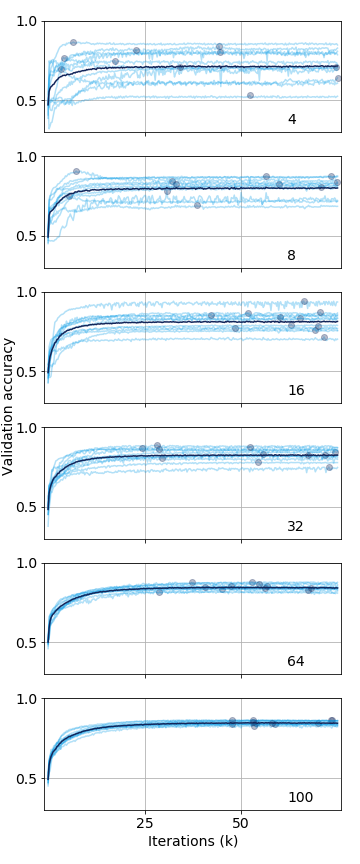
\includegraphics[width=3.5in]{./figures/learning}

\caption{Learning curves for each subset size (percent). In each sub-plot,
validation accuracy is plotted against number of training iterations. Each of
the repetitions is plotted in light blue, and the average across repetitions is
plotted in dark blue. Maximal validation accuracy in each course of training is
plotted as a light blue point.}

\label{fig_learning_curves}
\end{figure}

\subsection{Test accuracy as a function of subsample size}

For each training run, the weights from the training history with the maximal
validation accuracy were stored. The model was then assessed with these weights
against the held out test set, yielding 11 test accuracy estimates for each
proportion, as seen in Figure \ref{fig_test}. As expected, test accuracy
increased with sample size, reaching its maximal value at subsamples of 100 \%
($\sim$86 \% accuracy).

Though accuracy is far from chance even with only 4 \% of the data ($\sim$73\%
correct) it does increase precipitously between 4\% and 64\% of the data.
However, it reaches close-to-maximal accuracy already at a proportion 16 - 32\%
of the total data-set. To quantify the amount of data needed to reach 95\% of
the maximal accuracy, we fit a two-parameter logistic function to the accuracy
values across repetitions and sub-sample proportions (orange line in figure
\ref{fig_test}), fixing the saturation point of the function to be equal
to the mean accuracy at subsamples of 100 \% of the data. Inverting this
function, we find that 95\% of the maximal accuracy (approximately 82\%
accuracy) can already be achieved with 20\% of the data (dashed lines in
\ref{fig_test}).

\begin{figure}[!t]
\centering
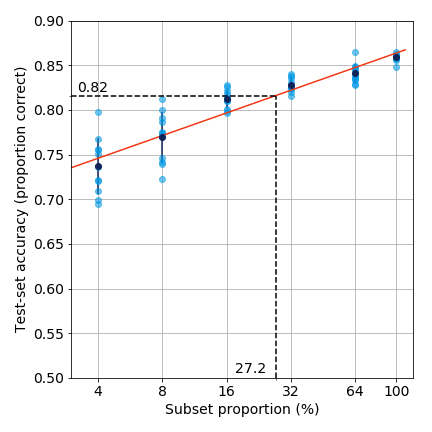
\includegraphics[width=3.5in]{./figures/test}

\caption{Accuracy on held out test set. Weights from the highest validation
accuracy during training were used to test accuracy on a held out test set. Dark
blue points are the means across 11 repetitions, with dark blue standard
deviation error bars. Orange line: a logistic curve model was fit to all of the
repetitions and sub-samples. According to this model, 95\% of maximal accuracy
($\sim$82 \% accuracy) can be achieved with 20.84\% of the data (dashed lines).}

\label{fig_test}
\end{figure}

\subsection{What explains variability between repetitions?}

Variability of test accuracy also diminished substantially with subsample size.
Differences in variability in the comparisons across different proportions.
These differences in variability could reflect two different factors: the first
is the subsample size, and the other is the degree of overlap between different
subsamples. For example, for 100 \% subsamples, variability reflects only the
random initial conditions of the network, because all subsamples of 100 \% are
identical.  Similarly, the overlap between different subsets in higher
proportions is likely to be larger than in smaller proportions. To evaluate the
effect of this overlap, we conducted a separate experiment in which a single
subset from 4\% group was used, and training was repeated 11 times using the
same set of images, to control for this effect. The learning curves from this
protocol are are shown in Figure \ref{fig_fourpercent}B, together with the
learning curves from random subsamples (Figure \ref{fig_fourpercent}B). The
learning curves have similar variance as when random subsets are used and the
maximal validation accuracy (Figure \ref{fig_fourpercent} C) does not differ
between these protocols. This indicates that variability in test-set accuracy
mostly relates to the size of the subsample, rather than to the amount of
overlap between different subsets.

\begin{figure}[!t]
\centering
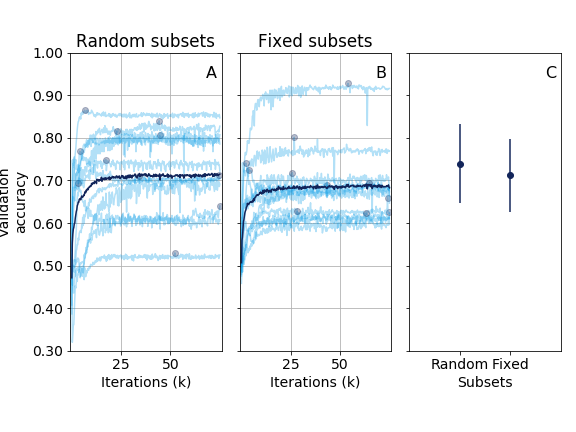
\includegraphics[width=3.5in]{./figures/fourpercent}

\caption{Learning curves of 4\% subset. {\bf A}: Random 4\% subsets of the whole
dataset chosen in each course of learning. {\bf B}: Replications of the same 4\%
susample were repeated in each course of training. {\bf C}: The average maximal
validation accuracies (across the 11 courses of training) are plotted for random
(left) and fixed (subsets) of 4\% each, with standard deviation error bars}

\label{fig_fourpercent}
\end{figure}

\subsection{The importance of a separate test set}

To assess the importance of the separate test set, we computed the difference
between the maximum validation accuracy and test set accuracy (Figure
\ref{fig_diff}). We find that though variability in this difference decreases
with larger sample size, there is no indication that this difference is larger
for smaller sample sizes. In addition, there seems to be no overall bias
indicating that the accuracy is systematically higher for the validation set,
relative to the test set. This indicates that in the training protocol that we
used, there was probably only minimal overfitting, or none at all.

\begin{figure}[!t]
\centering
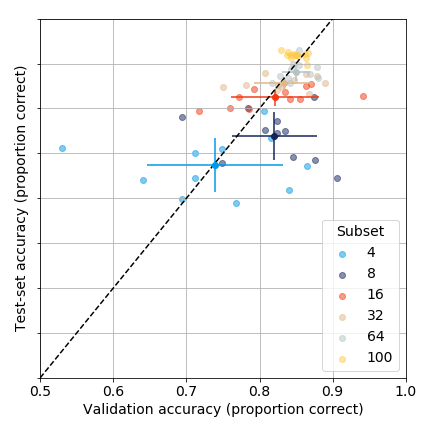
\includegraphics[width=3.5in]{./figures/diff}

\caption{Difference between validation and test accuracy. Each light colored
point represents a single course of training. The abscissa represents the
maximal validation accuracy achieved during this course of training, while the
ordinate represents the accuracy of the network in performing the classification
on a separate test set, using the same weights that resulted in maximal
validation accuracy. Solid colored points each represent the mean across 11
courses of training for each size subset, with standard deviation error bars. Dashed line indicates equality.}

\label{fig_diff}
\end{figure}
